\documentclass{article}

\usepackage{polski}
\usepackage[utf8]{inputenc}
\usepackage{graphicx}
\usepackage{xcolor}
\usepackage{float}
\usepackage{caption}
\usepackage{array}
\usepackage{pbox}

\newcommand\tab[1][1cm]{\hspace*{#1}}

\title{Dokumentacja projektowa}
\date{2018-03-18}
\author{Jędrzej Kozal}

\begin{document}

\begin{titlepage}
	\centering
	
\includegraphics[width=0.25\textwidth]{logo_pol_wroclaw.png}\par\vspace{1cm}
	{\scshape\LARGE Politechnika Wrocławska \par}
	\vspace{1cm}
	{\scshape\Large Miekkie metody obliczeniowe\par}
	\vspace{1.5cm}
	{\huge\bfseries Zastosowanie Sieci Bayesa do diagnozowania ostrych stanów zapalnych \par}
	\vspace{2cm}
	{\Large\itshape Filip Guzy\par}
	{\Large\itshape Jędrzej Kozal\par}
	{\Large\itshape Michał Leś\par}

	\vfill
	prowadzący\par
	Mgr inż.~Mariusz \textsc{Kozioł}

	\vfill

% Bottom of the page
	{\large \today\par}
\end{titlepage}

\tableofcontents
\newpage


\section{Wstęp}

Celem projektu jest zbadanie zastsowania Sieci Bayesa do automatycznego diagnozowania ostrych stanów zapalnych. 

\subsection{Wymagania projektowe}
W ramach projektu przewiduje się realizację:
\begin{enumerate}
	\item Analiza danych wejściowych
	\item Przygotowanie danych wejściowych - dychotomizacja, dyskretyzacja
	\item Podział danych wejściowych umożliwiający ocenę klasyfikatora
	\item Wyznacznie parametrów analizowanego zbioru potrzebnych do skontruowania modelu (określenie prawdopodobieństw a priori i wspólnych rozkładów prawdopodobieństwa)
	\item Przygotowanie modelu - Sieci Bayesa w konfiguracji QMR - i analiza wpływu topologii na uzyskane wyniki	
\end{enumerate}

\subsection{Wykorzystane narzędzia}
Do realizacji zadania wykorzystano środowisko Matlab, wraz z toolboxem BayesNet. Jako zbiór danych uczących wykorzystano zbiór Acute Inflammations Data Set dostępny w bazie UCI \cite{data set}.

\section{Podstawy teoretyczne}
W tej sekcji zostaną omówione teoretyczne aspekty problemu oraz przyjętych rozwiązań.

\subsection{Omówienie zagadanienia}

\subsubsection{Zbiór danych uczących}


\subsubsection{Interpretacja danych}
Pare słów o medycznym aspekcie i jakie dane analizujemy.

\subsection{Sieci Bayesa}

\subsubsection{Modelowanie probabilitystyczne}
W przypadku modelowania zależności między zmiennymi losowymi stosuje się wspólny rozkład prawdopodobieństwa (joint probabilty distribution, jpd). Dla dyskretnych zmiennych losowych stanowi ono tabelę z wszystkimi możliwymi kombinacjami wartości zmiennych. Dla 4 binarnych zmiennych losowych $A, B, C, D$ istnieje $2^4-1 = 15$ elementów tabeli. W ogólności liczba prawdopodobieństw $n$ zmiennych losowych w tabeli wynosi: $2^n - 1$. Funkcje wykładnicze bardzo szybko osiągają duże wartości, przez co modelowanie dla dużego $n$, może stanowić wyzwanie przez dużą liczbę paramterów.

\subsubsection{Definicja sieci Bayesa}
Sieć Bayesa to klasa modeli graficznych, w których do modelowania zależności między zmiennymi losowymi wykorzystuje się acykliczny graf skierowany. Wierzchołki grafu zawierają zmienne losowe, a krawędzie modelują zależności między zmiennymi losowymi. Wierzchołki połączone z wybranym wierzchołkiem przez krawedź wchodzącą nazywamy rodzicami (parent). Wierzchołki połączone przez krawędź wychodzącą nazywamy dziećmi (child). Wierzchołek nie posiadający rodziców nazywany jest korzeniem (root). Krawędzie grafu i jego struktura modelują zależności między zmiennymi losowymi, co pozwala na ogarniczenie ilości parametrów modelu.

\begin{figure}
\centering
	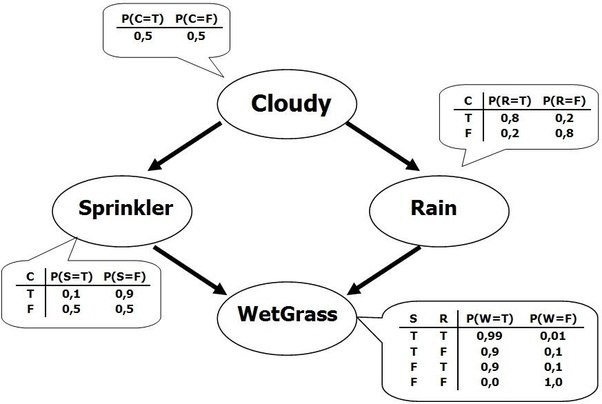
\includegraphics[width=0.80\textwidth]{net.jpeg}\par\vspace{1cm}
\caption{Przykładowa sieć Bayesa, modelująca wilgotność trawy, wraz z lokalnymi wspólnymi rozkładami prawdopodobieństwa. \\ źródło: https://towardsdatascience.com/introduction-to-bayesian-networks-81031eeed94e}
	\label{fig:net}
\end{figure}

Sieć Bayesa wykorzystuje założenie o niezależności zmiennych losowych do obliczania prawdopodobieństwa zmiennych losowych w wezłach, korzystając z prawdopodobieństwa wystąpienia konretnych wartości rodziców. 

Stosując regułę łańcucha dla prawdopodobieństwa, można zapisać wspólny rozkład prawdopodobieństwa jako:

\begin{equation}
	P(A, B, C, D) = P(A|B, C, D)P(B|C, D)P(C|D)P(D)
\end{equation}

Stosując założenie o niezależności $B$ od $C$ i $C$ od $D$ można tą samą regułę uprościć:

\begin{equation}
	P(A, B, C, D) = P(A|B, C, D)P(B|D)P(C)P(D)
\end{equation}

W ogólności dla Sieci Bayesa można zapisać:

\begin{equation}
	P(X_1, ... , X_n) = \prod_{i=1}^{n} P(X_i|Parents(X_i))
\end{equation}

Powoduje to znaczącą redukcję liczby parametrów modelu.

Przykładowa sieć Bayesa wraz z lokalnymi rozkładami prawdopodobieństwa została przedstawiona na rys. \ref{fig:net}. Poprzez podział tabel ze wspólnym rozkładem prawdopodobieństwa na mniejsze ilość paramterów modelu uległa zmianie z 15 do 18. Przy rosnącej ilości parametrów sieci Bayesa mogą przyczynić się do znaczącej redukcji liczby parametrów.

\subsubsection{D-separacja}

Pojęcie D-separacji może zostać wykorzystane do modelowania niezależności danych uczących ze zbioru. Jest ono ściśle powiązane ze strukturą sieci i opiera się na kilku zasadach. Przyjmijmy, że analizujemy dwie zmienne $X$ i $Y$. Zmienna losowa $Z$ znajduje się na ściężce $p$ w grafie między $X$ a $Y$.
\begin{enumerate}
\item Kiedy zmienna losowa $Z$ jest zdarzeniem warunkującym obliczanego prawdopodobieństwa (stanowi dowód, evidence) mówimy, że:
\begin{itemize}
 \item $Z$ jest zablokowane, jeżeli $p$ wchodzi do $Z$ od jego dziecka.
 \item $Z$ jest zablokowane, jeżeli $p$ wchodzi do $Z$ od jego rodzica i wychodzi od jego dziecka.
 \item $Z$ nie jest zablokowane, jeżeli $p$ wchodzi do $Z$ od jego rodzica wychodzi od jego rodzica.
\end{itemize}
\item Kiedy zmienna losowa $Z$ nie jest zdarzeniem warunkującym obliczanego prawdopodobieństwa mówimy, że:
\begin{itemize}
 \item $Z$ nie jest zablokowane, jeżeli $p$ wchodzi do $Z$ od jego dziecka.
 \item $Z$ nie jest zablokowane, jeżeli $p$ wchodzi do $Z$ od jego rodzica i wychodzi od jego dziecka.
 \item $Z$ jest zablokowane, jeżeli $p$ wchodzi do $Z$ od jego rodzica wychodzi od jego rodzica.
\end{itemize}
\end{enumerate}

$X$ jest niezależne od $Y$, jeżeli wszystkie możliwe ścieżki między $X$ a $Y$ w grafie są zablokowane.

$Z$ d-separuje $X$ od $Y$ (zapisywane: $X \perp_G Y|Z$), jeżeli wszystkie ścieżki między $X$ a $Y$ są zablokowane przez $Z$.

\subsubsection{Detekcja topologi sieci na podstawie danych uczących}

Ze względu na brak wiedzy dziedzinowej z zakresu medycyny, oraz braku możliwości konsultacji z ekspertem postanowiono wykorzystać metody pozwalające na nauczenie struktury sieci na podstawie zbioru uczącego.

W \cite{PhD} podano metody uczenia struktury sieci Bayesa. Wyróżna się dwie główne metody. Pierwsza z nich opiera się na maksymalizacji funkcji celu z wykorzystaniem maximum likelihood. Zaproponowano podejście w którym topologia sieci jest modyfikowana zgodnie z kierunkiem wzrostu maximum likelihood (hill climbing).

Drugą metodą opiera się na określeniu topologi na podstawie niezależności zmiennych losowych zbioru uczącego. Skierowany graf acykliczny jest nazywany I-mapą, jeśli:

\begin{equation}
	\forall_{X, Y, Z} (X \perp_G Y| Z) 	\Rightarrow  (X \perp_P Y | Z)
\end{equation}

Korzystając z zależności logicznej:

\begin{equation}
	p \Rightarrow q \Leftrightarrow \neg q \Rightarrow \neg p
\end{equation}

Aplikując poważyszy wzór dla sieci Bayesa można określić, że jeśli w domenowej dystrybucji P zmienne nie są niezależne to również nie powinny być niezależne w grafie (nie są d-separowane). W \cite{PhD} przedstawiono dokładny algorytm określania topologii sieci.

\newpage
\begin{thebibliography}{9}

\bibitem{data set}
J.Czerniak, H.Zarzycki, Application of rough sets in the presumptive diagnosis of urinary system diseases, 
Artifical Inteligence and Security in Computing Systems, ACS'2002 9th International Conference Proceedings, 
Kluwer Academic Publishers,2003, pp. 41-51 
\\\texttt{https://archive.ics.uci.edu/ml/datasets/Acute+Inflammations}

\bibitem{paper}
Ben-Gal I., Bayesian Networks, in Ruggeri F., Faltin F. \& Kenett R.,
Encyclopedia of Statistics in Quality \& Reliability, Wiley \& Sons (2007). 
\\\texttt{http://www.eng.tau.ac.il/~bengal/BN.pdf}

\bibitem{PhD}
Learning Bayesian Network Model Structure from Data, Dimitris Margaritis
May 2003, Carnegie Mellon University
\\\texttt{https://www.cs.cmu.edu/~dmarg/Papers/PhD-Thesis-Margaritis.pdf}

\bibitem{Towards Data Sience}
Introduction to Bayesian Networks, Towards Data Sience blog
\\\texttt{https://towardsdatascience.com/introduction-to-bayesian-networks-81031eeed94e}

\bibitem{bayesserver}
Baysian network software for Artificial Inteligence
\\\texttt{https://www.bayesserver.com/docs/introduction/bayesian-networks}

\end{thebibliography}
\newpage

\listoffigures
\newpage

\end{document}